\documentclass[10pt,conference,compsocconf]{IEEEtran}
\usepackage[T1]{fontenc}
\usepackage[utf8]{inputenc}
\usepackage{url}
\usepackage{comment}
\usepackage{graphicx}
\usepackage{multirow}
\usepackage{booktabs}
\usepackage{amsmath}

\usepackage{tikz}
\usetikzlibrary{fit}

\usepackage{acronym}
\acrodef{iaas}[IaaS]{Infrastructure as a Service}
\acrodef{SaaS}{Software as a Service}
\acrodef{PaaS}{Platform as a Service}
\acrodef{dag}[DAG]{directed acyclic graph}
\acrodef{vm}[VM]{Virtual Machine}
\acrodef{PM}{Physical Machine}
\acrodef{btu}[BTU]{billing time unit}
\acrodef{EC2CU}{EC2 Compute Unit}
\acrodef{HPC}{High Performance Computing}
\acrodef{unistra}{University of Strasbourg}
\acrodef{rv}[RV]{random variable}
\acrodef{pdf}[PDF]{probability density function}
\acrodef{cdf}[CDF]{cumulative distribution function}
\acrodef{mcs}[MCS]{Monte-Carlo simulation}
\acrodefplural{mcs}[MCS's]{Monte-Carlo simulations}

\newcommand*\rot{\rotatebox{90}}
\newcommand{\pmpc}[1]{$\pm#1\%$}
\newcommand{\etal}[1]{\emph{#1 et al.}}
\newcommand{\pc}[1]{$#1\%$}

\IEEEtriggeratref{17}

%\title{Modeling the accuracy of Monte-Carlo approach for Cloud based workflow
%  simulations.}

\title{Executing Batches of Jobs on Clouds: How to Accurately Predict the Reality?}


\author{\IEEEauthorblockN{Luke~Bertot 
			and Stéphane~Genaud 
			and Julien~Gossa}
	\IEEEauthorblockA{Icube-ICPS --- UMR 7357, Univeristé de Strasbourg, CNRS\\
		P\^ole API Blvd S. Bant, 67400 Illkirch\\
		email: \url{lbertot@unistra.fr}, \url{genaud@unistra.fr}, \url{gossa@unistra.fr}}
	}



\begin{document}

\maketitle

\begin{abstract}
  In the  cloud computing  model, cloud providers  invoice clients  for resource
  consumption. Hence, tools helping the client to budget the cost of running his
  application are  of pre-eminent  importance. To  that end,  a number  of cloud
  simulators have been  proposed by researchers. However, the  attempts to reach
  reliable  predictions are  hampered by  the opacity  regarding the  underlying
  hardware platform  and the  multi-tenant nature  of the  cloud which  make job
  runtimes both  variables and hard to  predict.  In this paper,  we investigate
  through two real  use-cases, which parameters are the most  influential in the
  prediction of the actual execution behavior in terms of cost and makespan.

  We consider the execution  of batch of jobs on a  actual platform, one example
  being a  bag-of-tasks and the other  one a workflow, whose  jobs are scheduled
  using typical  heuristics based on  the user  estimates of job  runtimes.  We
  propose an  improved simulation framework  based on the Monte-Carlo  method to
  study the  relationship between the  precision of  the user estimates  and the
  accuracy of the simulation results regarding  cost and makespan. Based on this
  stochastic process,  predictions are expressed as  interval-based makespan and
  cost.   We show  that imprecisions  in  user estimates  are most  of the  time
  largely amortized in the final predictions but still can capture real
  observations. Finally, we evidence the influence of the scheduling heuristics
  on the accuracy of the method.
 
\end{abstract}

\begin{IEEEkeywords}
cloud computing, computer simulation, monte carlo methods.
\end{IEEEkeywords}

\section{Introduction.}

Over the  last decade the advancement  of virtualization techniques has  lead to
the emergence of new economic and exploitation approach of computer resources in
the form of \ac{iaas}, one form of cloud computing. In this model, all computing
resources are made available on demand  by third-party operators and payed based
on usage.   The ability to provision  resources on demand provided  by \ac{iaas}
operators is mainly  used in two ways.  Firstly, for  scaling purposes where new
machines  are brought  online to  fulfill service  availability in  the face  of
higher load,  this approach  is used  for providing service  allows for  a lower
baseline cost while still being able to deal by spikes in demand by provisioning
machines  on  the go.   Secondly  for  parallelizing  tasks to  achieve  shorter
makespan as  equal cost,  this approach  is used  for scientific  and industrial
workload with  a clear end and  where runtime is heavily  dependent on computing
power.   This  approach  is  made  possible   by  the  pricing  model  of  cloud
infrastructure, as  popularized by  AWS\footnote{Amazon Web Services},  in which
payment  for computing  power, provided  as  \acp{vm}, happens  in increment  of
arbitrary length  of time, \ac{btu},  usually of  one hour. Running  two \ac{vm}
side by side for one \ac{btu} each costs the same as running one \ac{vm} for two
\ac{btu}, but every \ac{btu} started is owed in full.

From the client  perspective, provisioning an appropriate set  of resources in
order to  handle a set of  jobs is a difficult  task, for which tools  may be of
great help.   

The first type of tool is the scheduler. Compared to earlier distributed
computing systems  (e.g Grids),  the scheduling problem  statement in  the cloud
must be reformulated because of two fundamental novelties: firstly the size of the
infrastructure can be dynamically scaled, and secondly as economic cost can be
clearly measured, it naturally becomes an additional objective to the traditional
makespan  objective,  making  the   problem  multi-objective.   An abundance  of
heuristics have been  developed to adapt to the cloud  context, spanning a large
variety of assumptions about the setup.  The bi-objective issue is often tackled
by  combining the  cost and  makespan  metrics in  a  single one  or fixing  one
parameter as a constraint (deadline-  or budget- constrained schedule), while it
can be argued  that several solutions may be equally  interesting trade-offs and
it is up to the user to choose.  In~\cite{Su13} is proposed a strategy where VMs
belonging to a  Pareto front representing the most  cost-efficient resources are
used  in  priority  to  map  jobs.  Likewise,  in~\cite{Durillo14}  a  set  of
Pareto-optimal solutions are  proposed to the user, and this  is also the spirit
of our  own work.   Another discriminating criterion  between approaches  is the
assumption of  an \emph{online}  (or \emph{just-in-time}) or  \emph{offline} (or
\emph{static})  schedule,  on   the  type  of  workload   (independent  jobs  or
workflows),  the homogeneity  of  the ressources,  or the  way  they handle  the
multiple objectives.  Offline scheduling represents a large body of the research
works often based  on the adaptation of popular heuristics  aiming at minimizing
makespan in Grids.  For instance  the popular HEFT~\cite{Zhao2003} heuristic has
been  revisited in~\cite{LinL11},  which  adds the  ability  to scale  resources
depending on whether or not a task  can execute by its estimated finish time, or
is extended in~\cite{Li11cost-conscious} to select  slots with a balance between
runtime  and  cost.  However,  offline  scheduling  is often  evaluated  through
simulation while online scheduling is closer to the assumptions of practitioners
who evaluate  their ideas  on actual environments.   Online strategies  has been
early  proposed  for  bags-of-tasks,  to adress  the  problem  of  appropriately
provisioning                             the                            platform
(e.g~\cite{MarshallKF10,GenaudG11,DuongLG11,VillegasASI12}).  These  works share
many  commonalities, taking  especially  into account  some important  operating
system level details such as the boot time of a VM or the contention that occurs
if too many VMs are started simultaneously. We show in this paper that these are
influential factors to the prediction of the execution.
  
The second important  type of tool is a prediction  tool. Accurate prediction of
the  runtime of  scientific workloads  is  hampered by  multiple factors.  First
\ac{iaas}  operates in  a opaque  fashion, the  exact nature  of the  underlying
platforms are  unknown and  may slightly vary  for a given  type of  resource as
operators  complete their  data-centers  over  the years  with  new servers  and
equipment.   Secondly  cloud  systems  are  multi-tenant  by  nature  which adds
uncertainty due to  contention on network and memory accesses,  depending on how
\ac{vm}  are scheduled  and the  activity of  your \emph{neighbors}.   Even when
\ac{iaas} operators attempt to mask  these irregularities in computing power and
network  access by  guaranteeing a  minimum performance,  variability occurs  in
presence of \emph{less-than-noisy-neighbors} as it is not in the interest of the
\ac{iaas} operators to limit power  when available over the guaranteed minimums.
These factor add to the already  high difficulty of modeling job execution times
on network of computers as shown in~\cite{Lastovetsky05}.

To deal  with the inherent  unpredictability introduced by  opaque heterogeneous
platforms, the standard approach is to  consider jobs runtimes to be stochastic.
Every job can be modeled by a \ac{rv} that models the whole spectrum of possible
runtimes. These  \ac{rv} are  the basis required  for a  stochastic simulation.
Such  simulations   output  a  random   variable  of  the   observed  phenomenon
(\emph{makespan}  or  \emph{\ac{btu}}) which  in  turn  can  be used  to  create
intervals of possible  results with their assorted confidence. 

In this paper, we propose a stochastic method to enrich the classical prediction
based  on a  discrete-event  simulator, and  we study  the  conditions for  this
approach to be relevant. This study is  carried out on a real setting, described
in  section~\ref{sec:work-context},   where  the  applications   use-cases,  the
scheduler  and  the  experimental  observations are  presented.  The  stochastic
framework we propose is  then presented in section~\ref{sec:enriched-sim}, and
is evaluated in section~\ref{sec:eval}. We finally conclude by discussing the 
improvements and the limits of the approach.


\section{Work Context}
\label{sec:work-context}
\begin{figure*}
	\centering
	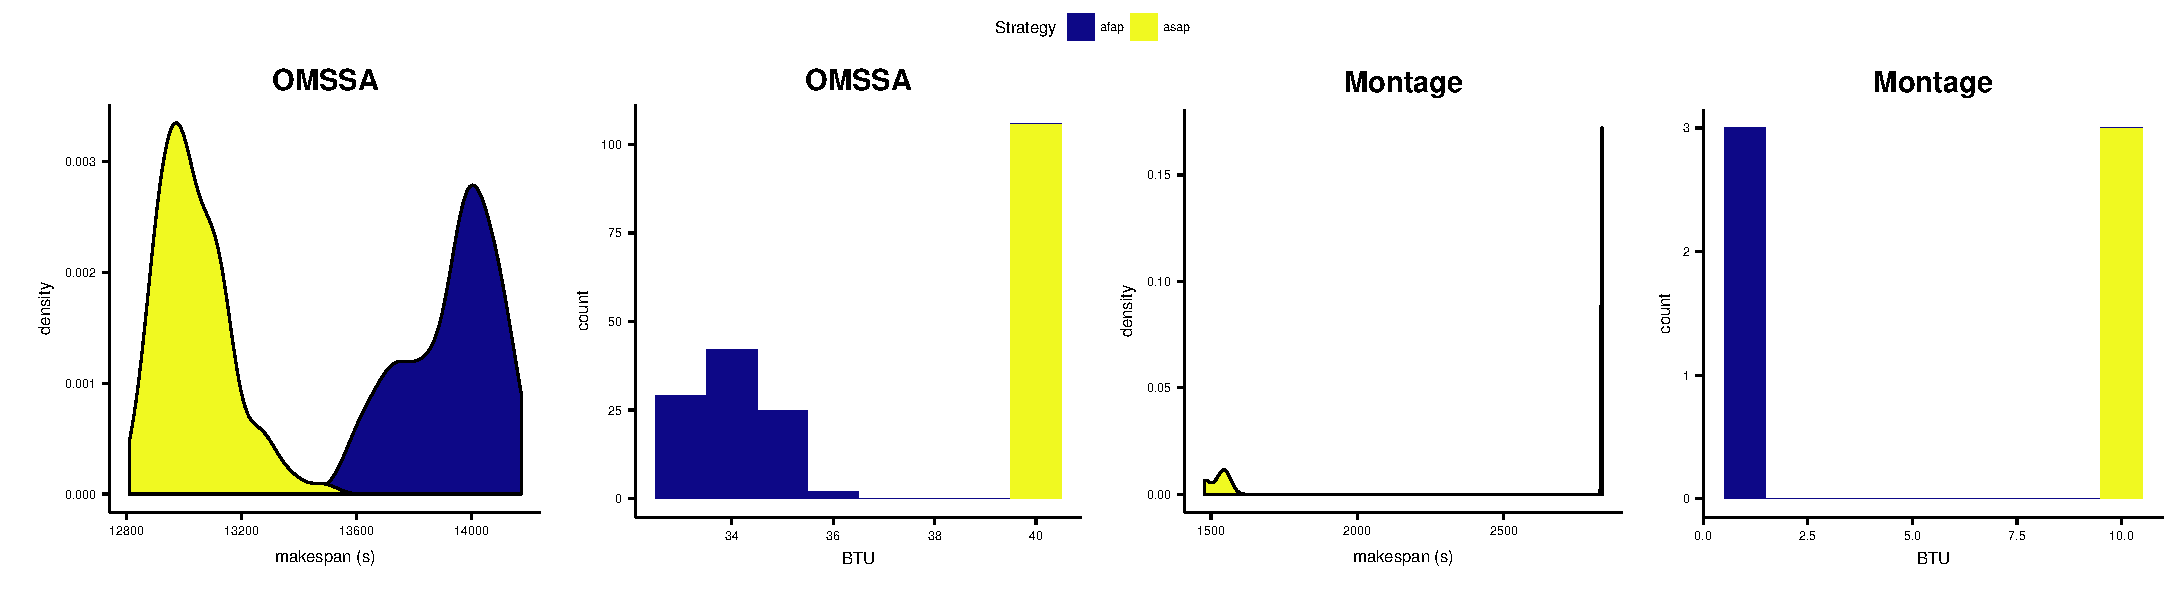
\includegraphics[width=\textwidth]{gfx/real_plot.pdf}
	\caption{Makepsan and BTU count distribution for OMSSA and Montage
	runs\label{fig:realbrs}}
\end{figure*}
\subsection{Schlouder}
In the recent years, we have developed a client-side job broker for IaaS clouds
called Schlouder~\cite{Michon17}. This broker is able to submit on behalf of its
user a  batch of  jobs, be  it a  set of  independent jobs  or a  workflow.  The
broker main role is to schedule the set of jobs onto a set of cloud resources,
which the broker can  scale up or down depending on  a \emph{strategy} chosen by
the user.  Technically, the broker connects  to the cloud management system (for
instance OpenStack) to  instruct how the infrastructure  should be provisioned
and  then assigns  the jobs  to  the resources  using the  Slurm job  management
system. 

Applications are  submitted to Schlouder  as job  batches. Each job  is provided
with  a  \emph{user estimate}  of  the  runtime, and  if  the  application is  a
workflow, the list of dependencies. Schlouder uses just-in-time scheduling where
jobs  are  assigned   to  \acp{vm}  as  soon  as  all   their  dependencies  are
satisfied.  We call  \emph{strategy} the  heuristic  used by  Schlouder to  make
provisioning and scheduling  decisions.  A dozen of strategies  and variants are
available to  the user (details can  be found in~\cite{GenaudG11}), of  which we
will use  two in this  paper. Strategies  provision \acp{vm} and  schedules jobs
based on the user estimates of the runtime. Notice that the jobs' real runtimes,
called \emph{effective runtimes},  may differ from the estimates,  but this does
not change the initial scheduling decision regarding to which resources the jobs
are assigned.

As mentioned in introduction, as no solution usually dominates the other in all
objectives, we leave to the user a choice of strategies which will favor one or
the other objective (cost or makespan). These two main strategies proposed by
Schlouder are:
\begin{itemize}
\item ASAP (or \textit{as soon as possible}): schedules the job immediately onto
  an idle VM, or immediately provisions a new VM to start the job if no idle VM 
  is available.  Hence this strategy tries to minimize the makespan
  of the job batch execution.

\item AFAP (or \textit{as full as  possible}): schedules each job in priority to
	an already  available resource where  the remaining time  before a new
	\ac{btu} is started is greater or equal to the job estimated runtime.
	By solving this bin-packing problem, this strategy tends to minimize the
	monetary cost of the batch execution.
\end{itemize}
In the following, we will evaluate the real executions against the backdrop of these two
strategies.

\subsection{Experimental Set-up and Test Applications}\label{sc:setup}

To evaluate Schlouder performance we carried out multiple executions of
common scientific applications. The execution traces for those runs where
collected into an archive. This backlog of real execution is the benchmark
against which our simulation performance will be evaluated. The applications
used are:

\begin{itemize}
	\item Montage\cite{montage2009}, the Montage Astronomical Image Mosaic
		Engine, is designed to splice astronomical images. The structure
                of this application is a fork-join type workflow. This
                application  is extremely data intensive with a
		\emph{commuication-to-computation} ratio superior to $90\%$.
	\item OMSSA\cite{Geer2004}, the Open Mass-Spectrometry Search Algorithm, 
		is used to analyze mass-spectrometer results. The application is
                parallelized as a bag-of-tasks, \textit{i.e} as a number of
                independent parallel jobs. This application is
		computation intensive with a
		\emph{communication-to-computation} ratio under to $20\%$.
\end{itemize}
\begin{comment}
\begin{figure}
	\resizebox{0.5\textwidth}{!}{%
		\usetikzlibrary{fit,arrows}
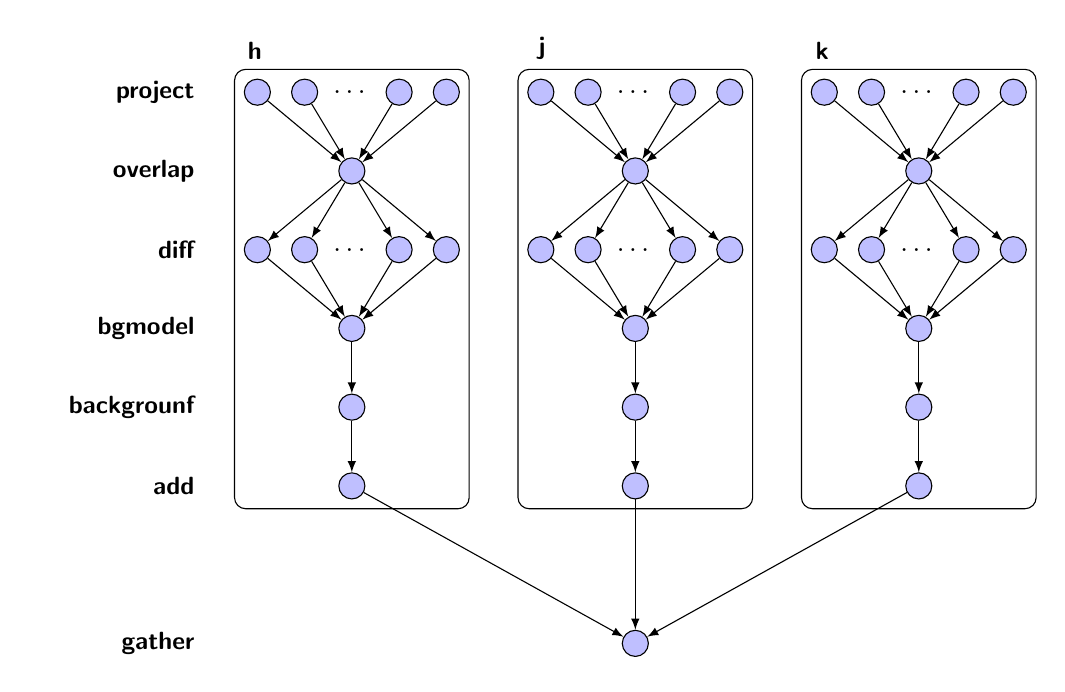
\begin{tikzpicture}[x=6mm,y=-10mm,
task/.style={%
 fill=blue!25,
draw,circle
},
level/.style={%
  font={\sffamily\bfseries\color{black} \fontsize{9pt}{12}\selectfont},
  align=right,
  text width=20mm
},
dot/.style={%
circle
}
]
%levels
\node[level] at (0,0)(Lproj){project};
\node[level] at (0,1)(Loverlap){overlap};
\node[level] at (0,2)(Ldiff){diff};
\node[level] at (0,3)(Lbgm){bgmodel};
\node[level] at (0,4)(Lbg){backgrounf};
\node[level] at (0,5)(Ladd){add};
\node[level] at(0,7)(Lgather){gather};
%%Gather node
\node[task,shift={(9,0)}]at(2,7)(gather){};
%%Loop HJK
\foreach \n [count=\i from 0] in {h,j,k}
{%
\begin{scope}[shift={(3+6*\i,0)}]
% 1 node per group
\node[task]at(2,1)(\i_overlap){};
\node[task]at(2,3)(\i_bgm){};
\node[task]at(2,4)(\i_bg){};
\node[task]at(2,5)(\i_add){};
%% 4 node per group
\foreach \y in {0,1,3,4}
{%
\node[task]at(\y,0)(\i_p_\y){};
\node[task]at(\y,2)(\i_d_\y){};
\draw[-{latex}](\i_p_\y)--(\i_overlap);
\draw[-{latex}](\i_overlap)--(\i_d_\y);
\draw[-{latex}](\i_d_\y)--(\i_bgm);
}
%%4 groups elipsis
\foreach \y in {0,2}
{%
\node[dot]at(2,\y){\ldots};
}
%%single deps
\draw[-{latex}](\i_bgm)--(\i_bg);
\draw[-{latex}](\i_bg)--(\i_add);
%%HJK boxes
\node[rounded corners,draw,fit=(\i_add)(\i_p_0)(\i_p_4),label={[font={\sffamily\bfseries\color{black}\fontsize{9pt}{12}\selectfont}]110:\n}]{};
\end{scope}
%% Gather deps
\draw[-{latex}](\i_add)--(gather);
}
\end{tikzpicture}
		}%
	\caption{Montage workflow diagram.}\label{fig:montage}
\end{figure}
\end{comment}

These two applications were executed using Schlouder on a private cloud.  We set
up a 96 core cloud based on four identical  dual $2.67GHz$ Intel Xeon X5650
servers with KVM based virtualization  and an Openstack cloud-front (first
2012.1, and later 2014.2). This cluster was exclusive to our usage and special
attention was given to never overload the system.

\subsection{Experimental Observations}

Schlouder execution traces contain several useful metrics including, but not
limited to, the \ac{vm} start dates, boot time, shutdown times and tasks
assigned, and the task start date and effective runtimes. We are interested in
two macro metrics, the makespan and the cost.  The makespan is the time elapsed
between the submission of the first job and the completion of the last completed
job. The cost is measured as a number of \acp{btu}. Since our experiments have a
single \ac{vm} type we counted one \ac{btu} per \ac{vm} per started hour to
match the most common pricing on the cloud. Table~\ref{tab:nbruns} gives an
overview of the executions in the archive used in this paper. We observe
variability on the makespan due to the variability of individual job effective
runtime.
\begin{table}
	\centering
	\caption{Overview of archived executions}\label{tab:nbruns}
	\begin{tabular}{llrcc}
		\toprule
		Application&Strategy&\#runs&BTU count&Makespan ($s$)\\
		\midrule
		\multirow{2}{*}{OMSSA}&ASAP&106&40&12811 -- 13488\\
				      &AFAP&98&33 -- 36&13564 -- 14172\\
		\midrule
		\multirow{2}{*}{Montage}&ASAP&3&10&1478 -- 1554\\
					&AFAP&3&1&2833 -- 2837\\
		\bottomrule
	\end{tabular}
\end{table}


Figure~\ref{fig:realbrs}  presents the  distribution of  makespans and  \ac{btu}
counts over  more than  200 runs.  This exposes the  behaviour exhibited  by the
different strategies. ASAP  appears to finish faster in the  most cases and AFAP
is less costly. But  these optimizations come at the cost  of instability on the
dimension they  aim to  optimize. ASAP uses  a high number  of \ac{btu}s  but this
number of \ac{btu}s  is stable, whereas AFAP uses a lower number of \ac{btu}s  
but this number of \ac{btu}s is  more variable.  When
looking at the makespan, we take note of how the different strategies affect the
skewness of  the overall distribution. The  positive skew seen on  ASAP suggests
that even though  the strategy globally produces  shorter makespan, perturbations
are more likely  to extend the makespan, whereas AFAP  makespans are more spread
out and skews negatively.

All the behaviours discussed in this section are due to the specifics of the
provisioning and scheduling strategies. In the case of AFAP and ASAP a thorough
analysis could probably expose the strategies instabilities, but that would not
be possible on more complex and dynamic strategies. In the following sections we
choose to consider strategies as black boxes to show that through simulation 
we are able  to obtain an accurate prediction of the distribution of our runs
and of the biases of our strategies.

\section{Enriched Simulation Framework}
\label{sec:enriched-sim}

\subsection{SimSchlouder}

As a follow-up on our work on Schlouder we developed SimSchlouder, a simulator
reimplementing the behaviour of Schlouder. Integrated to Schlouder, this
simulator allows the user to request an estimate of the makespan and the cost
before choosing a strategy for a real run. SimSchlouder includes the same
strategies as Schlouder, and as its real-world counterpart it is easily
extendable with new strategies. SimSchlouder is based on SimGrid~\cite{simgrid},
a framework to build discrete event simulators of distributed systems such as
Grids, Clouds or HPC systems. SimGrid has been chosen as the simulation engine,
for the versatility of its interfaces, and above all, for its well studied
accuracy against reality (e.g~\cite{StanisicTLVM15,VelhoSCL13}).


For the purpose of this paper, we classify the inputs required by SimSchlouder
in two categories. The first category is the operator inputs, which describe the
hardware platform and the cloud configuration. Internally, they are fed to the
SimGrid core and the \ac{iaas} simulation layer. The second category is the end
user inputs. They describe the workflow to simulate, the submission dates of
each job, the runtime prediction that would be provided to Schlouder.
Additionally for the purpose of the simulator, a user can choose to supply
effective runtimes to match, communication to simulate, or alternative boot
times for the \acp{vm}. Those additional inputs are used to alter the sequence
of events simulated without interfering with parameters that would change the
provisioning or scheduling decisions made by SimSchlouder, eg.\ having a job
overrun its runtime without changing the corresponding user prediction.

As exposed above, the variability of real executions suggests that a simulation,
even if it was  perfectly accurate, would capture only one of the set
of possible reals  executions. We will show later that  the simulation is indeed
very   accurate  when   the  user   estimates  are   close  to   the  effectives
runtimes. However,  to  provide the user  with a broader view  of how
his/her real executions could behave with job runtimes variability,  we should enrich the simulation framework
with some form of stochastic prediction.

\subsection{Monte-Carlo Simulation}\label{sec:MCS}

Stochastic  simulations are  computationally more  expensive than  deterministic
ones. In stochastic simulations inputs  become random variables representing the
distribution of possible values for the parameters. In the context of stochastic
\ac{dag} it has  been shown that computing the  makespan distribution requires
multiple derivations and  integrations~\cite{Ludwig01,Li97}. Monte Carlo methods
allow us to side step these computational difficulties. This method was proposed
for PERT  graphs in 1967~\cite{Slyke63}, and  in the recent year  in the context
\ac{dag} scheduling~\cite{Canon10,Zheng13}.

\aclp{mcs} (\acs{mcs})\acused{mcs}  work by  repeatedly drawing  input variables
and using  them in deterministic simulations  to obtain samples of  the possible
results. Once enough samples have been computed, traditional fitting can be used
to characterize the resulting random variable.  In our case, we will draw values
of  the  effective runtimes  of  the  individual  jobs,  and we  obtain  through
simulation samples of makespans an BTU counts.

%\paragraph{Method} 
Suppose an  application consisting of  $n$ jobs,  independent or organized  as a
workflow.  The simulation engine SimSchlouder  takes as input the user estimates
$T_1, \ldots , T_n$ for the job runtimes, schedules the jobs and finally outputs
the makespan $M$ of the whole batch.  The user estimates might be inaccurate,
and  we describe  hereafter  a method  to characterize  the  impact of  repeated
imprecisions (on each  job runtime) on the final makespan.   We have developed a
\ac{mcs} tool to  compute a confidence interval around the  makespan produced by
simulation.  Let us sketch the overall process (see Fig~\ref{fig:mc-process}):
\begin{itemize} 
\item from  the set of  specified runtimes  $\{T_i\}$, the system  generates $s$
  sets  of perturbed  runtimes $\{T_i^1\},  \ldots, \{T_i^s\}$.   Each perturbed
  runtime  is a  random  value  uniformly drawn  around  $T_i$  (to be  precised
  later). We call \emph{realization} each such random draw of a set of perturbed
  runtimes.
\item a simulation  is run for each realization, producing  a makespan $M^i$ and
  BTU count sample for each,
\item a  normal distribution ${\cal  N}(\mu,\sigma)$ is fitted on  the different
  makespan values.
\end{itemize}
\begin{figure}
	\centering
	\resizebox{0.5\textwidth}{!}{%
		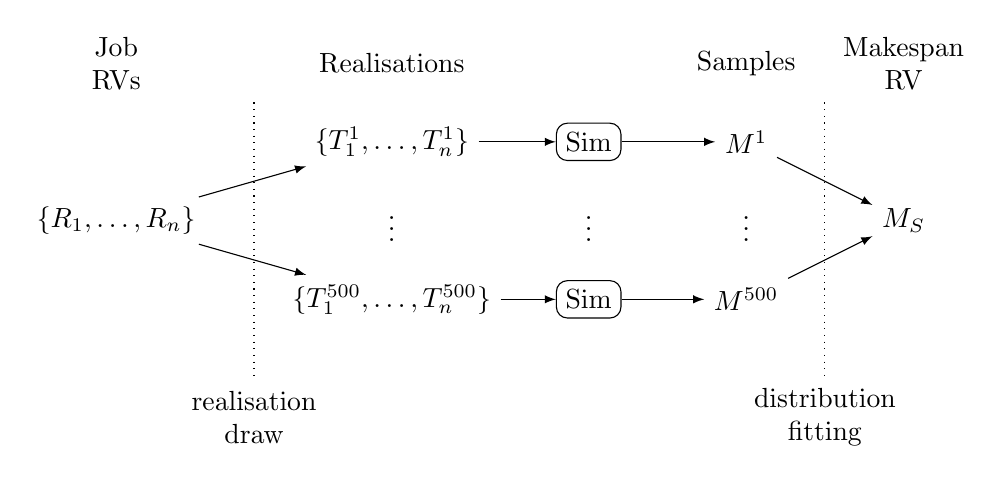
\begin{tikzpicture}[
sim/.style={%
draw, 
rounded corners
}
]
%% Origin node
\node[align=center]at(0,2){Job\\RVs};
\node at(0,0)(orig){$\{R_1,\ldots,R_n\}$};
%% Realisations
\node at(3.5,2){Realisations};
\node[]at(3.5,1)(pert1){$\{T_1^1,\ldots,T_n^1\}$};
\node at(3.5,0){\vdots};
\node at(3.5,-1)(pert5){$\{T_1^{500},\ldots,T_n^{500}\}$};
\draw[-{latex}](orig)--(pert1);
\draw[-{latex}](orig)--(pert5);
%%
\node[sim]at(6,1)(s1){Sim};
\node[sim]at(6,-1)(s5){Sim};
\node at(6,0){\vdots};
\draw[-{latex}](pert1)--(s1);
\draw[-{latex}](pert5)--(s5);
%% Makespans
\node at(8,2){Samples};
\node at(8,1)(M1){$M^1$};
\node at(8,-1)(M5){$M^{500}$};
\node at(8,-0){\vdots};
\draw[-{latex}](s1)--(M1);
\draw[-{latex}](s5)--(M5);
%% Consolidation
\node[align=center]at(10,2){Makespan\\RV};
\node at(10,0)(r){$M_S$};
\draw[-{latex}](M1)--(r);
\draw[-{latex}](M5)--(r);
%%phases
\node[align=center]at(1.75,-2.5)(df){realisation\\draw};
\draw[dotted](1.75,1.5)--(1.75,-2);
\node[align=center]at(9,-2.5)(df){distribution\\fitting};
\draw[dotted](9,1.5)--(9,-2);
\end{tikzpicture}

		}
\caption{Overview of the Monte-Carlo process: $500$ realizations are generated
by drawing and adding a perturbation to each job runtime of the provided
runtimes set, every simulation is then simulated, the resulting makespans
samples are fitted into the final result.}\label{fig:mc-process}
\end{figure}
Fitting is done to a normal distribution because, in essence the makespan is the
sum  of the  runtimes of  the jobs  on the  critical path  of the  schedule.  To
measure the impact  of the runtime perturbation on the  makespan, we compute the
range $[\mu-2\sigma;\mu+2\sigma]$ (that is  a 95\% confidence interval) relative
to  the mean  $\mu$. 

%% Free floating graphs mus be declared a page in advance
\begin{figure*}
	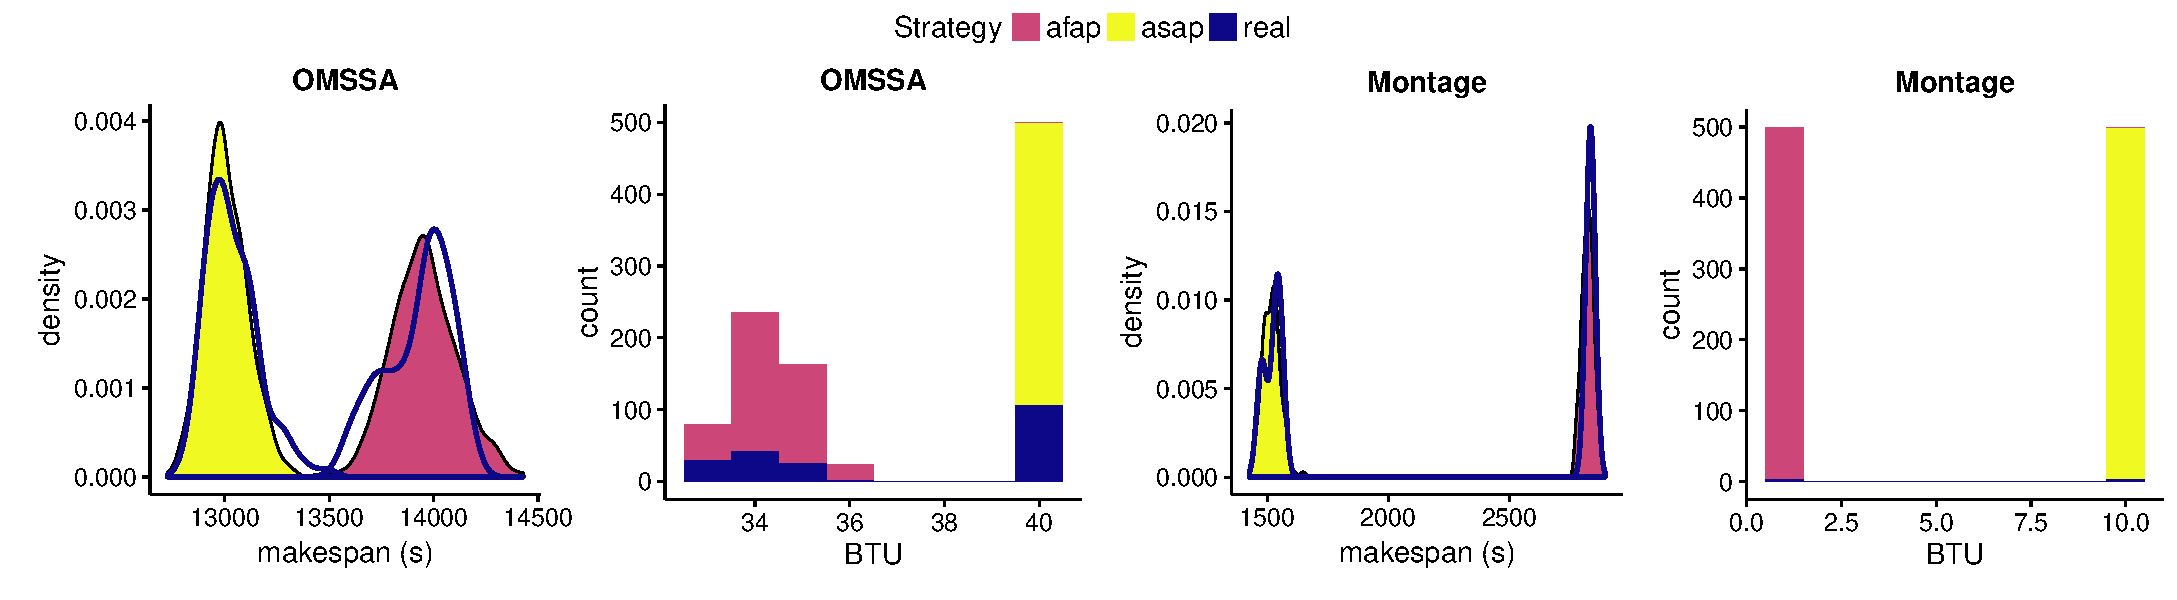
\includegraphics[width=\textwidth]{gfx/fit_plot.pdf}
	\caption{Makespan and BTU count distribution for OMSSA and Montage Monte
	Carlo Simulation compared to reality at 10\% perturbation
	level.}\label{fig:fit}
\end{figure*}

\subsection{Input Modeling}\label{sec:im}

Core  to the  \acl{mcs} is  the accuracy  of our  job runtimes  inputs. Given  a
precise simulator and enough samples, the \ac{mcs} will return a precise result,
but this  result corresponds to  the reality described  by the inputs.  In other
words, for the result to be a good  predictor of the reality, the inputs must be
a good descriptor of reality.

Hence, we seek  to determine which is  the range of acceptable  input values for
the  \ac{mcs} to  produce accurate  enough predictions  (in terms  of confidence
interval),  and we  term this  research \emph{input  modeling}.  Answering  this
question will tell the  acceptable margin of error in the  user estimate for the
method to be relevant.
An ideal  model would present  an individual distribution  for every job  in the
workflow, and such a distribution would require a deep understanding of the jobs
computation, communication, and  of the underlying platform.  In  real life such
modeling  is not  practical  as the  underlying platform  is  usually not  known
precisely, and  the user might  not be very  familiar with the  application. For
this reason, despite having ourselves a  comprehensive archive, we choose to use
a more generic model.

As discussed in Section~\ref{sec:MCS}, for the purpose of our \ac{mcs} we
consider job runtimes as a base runtime on which is applied a perturbation.  The
extent of this perturbation is called the \emph{perturbation level} and is
denoted $P$. Though the base is determined job per job, the perturbation level
is set simulation wide. We set the effective runtime of a job $i$ within the
$n$\textit{-th} simulation of an \ac{mcs} to: \[T_i^n = T_i * (1+r_i^n)\] with
$r_i^n$ the perturbation value drawn between $[-P;+P]$.

As we  will see  in Section~\ref{sec:sa},  the parameters $T_i$  and $P$  have a
great influence on the \ac{mcs} results.  Our findings are that the best results
are obtained by  taking as $T_i$ the average effective  runtime observed for job
$i$ for a given  strategy. This corresponds to the guess of a knowledgable user.
Regarding  the simulation  wide perturbation level  $P$, we found  that the best
setting  is the average  of the worst relative deviations for all jobs in the
workload:

\[P = \underset{i}{\textrm{mean}}(\delta{}_i)\]
\[\delta{}_i = \max_n\left(\frac{R_i^n-\textrm{mean}(R_i)}{\textrm{mean}(R_i)}\right)\]
with $R_i^n$ the observed effective runtime for job $i$ during execution $n$. 

For OMSSA, the perturbation level given by this methods is roughly 10\% for both
strategies. For Montage  our calculated perturbation level is  20\% when looking
at ASAP  executions and  5\% when  looking at AFAP  executions. We  believe this
difference can be partially  explained by the low number of  montage runs in the
archive. As such we additionally ran a Montage simulation using the 10\% 
perturbation level calculated using the OMSSA executions.

For  each  application and  strategy  we  also  perform a  single  deterministic
simulation  using the  raw base  value  with 0\%  perturbation. This  simulation
serves as  reference when  evaluating the strategies  behaviour when  faced with
perturbations.

\section{Evaluation}
\label{sec:eval}

\begin{figure*}
	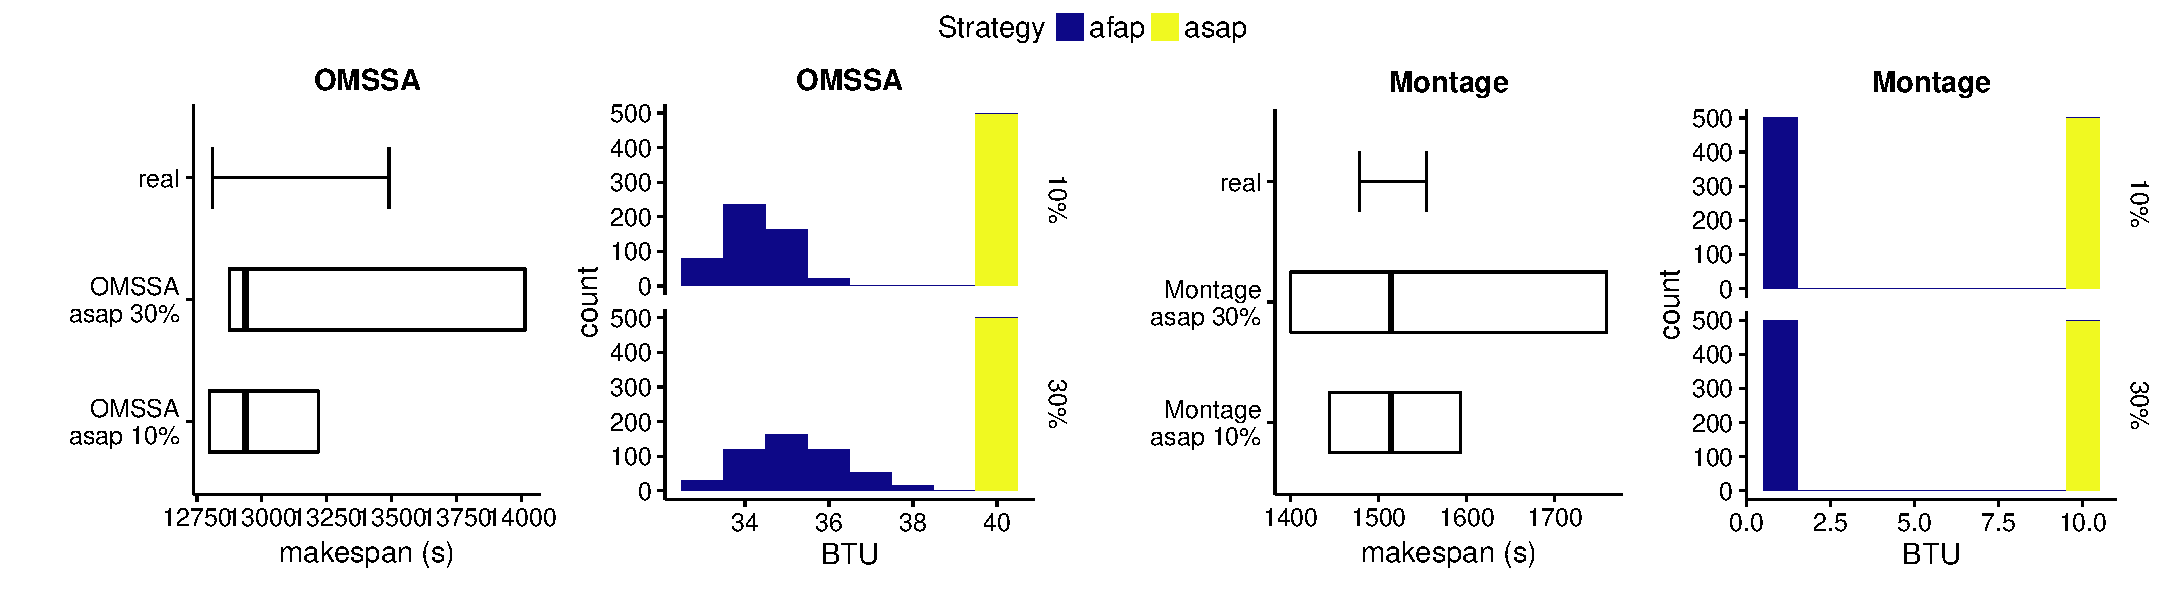
\includegraphics[width=\textwidth]{gfx/int_plot.pdf}
	\caption{Makespan intervals and BTU count distribution for OMSSA and 
	Montage at different perturbation levels. In makespan interval graph the 
	box represent the 95\% confidence interval resulting from the \acs{mcs},
	and the crossbar the results of a single unperturbed simulations us 
	average job times.}\label{fig:int}
\end{figure*}

\begin{table}
	\centering
	\caption{Makespan and BTU capture rate depending on confidence interval
          (CI) for a 10\% perturbation level}\label{tab:fit}
	\begin{tabular}{llccc}
		\toprule
		Application&Strategy&\multicolumn{2}{c}{Makespan (Size of CI)}&BTU\\
                           &         & CI 95\% & CI 99\% &\\
		\midrule
		\multirow{2}{*}{OMSSA}&ASAP&  90\% (3\%)&  98\% (5\%)& 100\%\\
				      &AFAP&  92\% (4\%)& 100\% (6\%)& 100\%\\
		\midrule
		\multirow{2}{*}{Montage}&ASAP& 100\% (2\%)& 100\% (4\%)& 100\%\\
					&AFAP& 100\% (1\%)& 100\% (2\%)& 100\%\\
		\bottomrule
	\end{tabular}
\end{table}
\subsection{Prediction Quality}\label{sec:pq}

We evaluate the  validity of our simulation based on  two different factors, the
\emph{makespan capture  rate} and  the \emph{BTU capture rate}.   The makespan
capture rate is the percentage of  real makespans which fall into the confidence
interval generated by fitting the  makespans of our individual simulations using
a Normal distribution, as  discussed in Section~\ref{sec:MCS}.  Unless specified
otherwise we  use a standard 95\%  confidence interval of width  $4\sigma$.  BTU
capture rate is the ratio of BTU counts found in the simulation to the BTU
counts observed  during our  real runs.  Figure~\ref{fig:fit} shows  results for
\acp{mcs} using  the input  model presented  in the previous  section at  a 10\%
perturbation level.

Table~\ref{tab:fit}  summarizes the  results obtained  with a  10\% perturbation
level. Along with the makespan capture rates is included in parenthesis the size
of the confidence interval relative to  the average makespan.  With our model we
are able to  capture 90\% of real executions  in ASAP and 92\% of  real AFAP run
for OMSSA\@.  These intervals  span 7  and 10  minutes respectively  whereas the
results in our archive  spread over 10 and 11 minutes.   Using a 99\% confidence
interval results in  better capture rates of  100\% for AFAP and  98\% for ASAP,
but also  in wider intervals  of 15 minutes.  Such  an interval increase  may be
seen as having little impact, like in  our OMSSA use-case exhibiting 3 to 4 hour
runs. Probably  is this choice  of the confidence  interval best let  to the
user.

For cost prediction our enriched  simulation finds exactly the same possibilities
as experienced in reality, though in  the case of AFAP, repartition favors higher
BTU counts slightly more than observed in our backlog.

Working on Montage when using \acp{mcs} with the perturbation level of its
respective strategy, as seen in Section~\ref{sec:im}, capture rate is 100\%
across all strategies. This capture rate is maintained when using the 10\%
perturbation obtained using the OMSSA archive. In this cases the intervals span
from 1.5 to 2.5 minutes for AFAP and ASAP respectively on workflow lasting from
47 to 25 minutes. Because Montage has a sub 1 hour runtimes BTU counts are
naturally stable, which is perfectly assessed by our simulations.

The results shown in  this section show that provided a  good description of job
runtimes our simulator will provide  good predictions of the possible executions
of this runs. However,  thought we strived to keep our  input modeling as simple
as possible, the  benefits of hindsight provided by the  archive means that only
the users most knowledgeable about their  workload and the targeted platform can
hope to achieve such predictions.  In Section~\ref{sec:lim}, we will discuss the
limits we experienced with this approach. In the next section we show by comparing
different \acp{mcs}  that we are able  to study the behavior  of the strategies
when confronted with different applications and perturbation levels.


\subsection{Strategy analysis}\label{sec:sa}

In our method the perturbation is meant to capture all sources of uncertainties
that could affect a job runtime, noisy neighbors, memory access contention,
cache misses, or even variations in the underlying platform. This has allowed us
to bring all these uncertainties under one dimension, but it should be noted that
we could achieve similar results by having a different \ac{mcs}, draw different values
of network bandwidth, cpu-speed, or any other uncertain parameters for each
individual simulation. Our one-dimensional approach is much easier to implement
but at the cost of making the perturbation level more difficult to construct.

In this section we  continue to base our user estimates  on the average runtimes
of the  jobs, as a  knowledgable user  would, but consider  that we do  not know
which perturbation  level is appropriate for the given platform  and application
strategy.   In such  a  situation a  user  would be  interested  on testing  his
application with different perturbation levels.

Figure~\ref{fig:int} presents  the results  of such simulations  for a  10\% and
40\% perturbation level.  On the  makespan interval graphs (left subfigures) the
boxes represent the span  of the capture interval and the  crossbar inside a box
represents   a   single   0\%   perturbation  simulations   done   outside   the
\ac{mcs}. Comparing  the interval  of perturbed  simulation to  this unperturbed
simulation allows us to view the effect  of perturbation on the strategy. On top
in  these subfigures,  are presented  for  reference the  interval spanning  the
minimum and maximum observed makespans over all runs.

These effects are most noticeable in the leftmost graph of Fig.~\ref{fig:int}
showing the makespan intervals obtained for OMSSA at 40\% and 10\% perturbation
levels. With the increase of the perturbation level the intervals get naturally 
wider, but the average makespan, by definition the center of the capture 
interval, also gets higher. On OMSSA this happens to the extent that the lower 
bound of our interval at 40\% is higher than the lower bound at 10\%.
This shows that ASAP, a strategy geared towards reducing the makespan regardless
of cost, is not as effective when scheduling bag-of-tasks in environments where
job runtimes might vary widely.  This is also true to a certain extent when
scheduling workflows. As seen in the third graph of Fig.~\ref{fig:int} the
average runtime for Montage also increases slightly with the perturbation level.

When looking at cost, these simulations show that with AFAP, as
perturbation level increases, low BTU count runs become less likely to occur and
higher BTU counts become possible. This is not the case for ASAP, or in context
where the application is clearly under an hour.

This approach to analyzing strategies and their interactions with workflow has
the notable advantage of not requiring complete understanding of a strategy, as
long as a correct implementation of the strategy is available in the simulator,
it can be considered a black box. The enriched simulation allows the user to
witness its behavior against any workflow or variability.


\subsection{Advantages and limitations of the enriched simulation}\label{sec:lim}

Thanks to our backlog of executions, we were able to build a trustworthy model
of how the applications behaved on our platform. Our ability to check repeatedly
our simulation against reality has allowed to test multiple ways to models our
inputs and multiple options on what to simulate. 

First we found that  for our purposes the \ac{mcs} did  not require thousands of
deterministic simulations to  be successful. When used in other  domains such as
physics \acp{mcs} are often used with up from 20\,000 deterministic simulations,
but  the size  of the  input  distribution is  usually much  larger. The  result
presented  in this  paper were obtained using  500 simulations per \ac{mcs}.  By
keeping  the results  of the  individual simulations  ordered, we  were able  to
determine  that by  the hundredth  simulation the  average makespan  was already
precise to the second, with its value hardly changing by the addition of the 400
next  simulations. The  standard  deviation used  to compute  the  width of  the
makespan interval was less stable, but still showed strongly diminishing returns
past the 100th simulation mark.

As discussed in Section~\ref{sec:MCS}, \aclp{mcs} replaces a stochastic
simulation by repeated execution of deterministic simulations of the same
phenomenon on random samples of the possible inputs. It is critical that the
operators inputs to the simulation be correct within the deterministic simulations.
This include for example the correct simulation of boot times, and correct
reimplementation of strategies. Ideally, the deterministic simulator is able to
properly reproduce real runs when fed with all the relevant information. In cases
where some external parameter is also unstable or unpredictable, it can also be
made part of the \ac{mcs} to be randomly drawn at each iteration.

Increasing the perturbation level will not always increase the predictions
capture rate. To illustrate this we added the intervals of observed real
makespans to the relevant graphs in Figure~\ref{fig:int}. On the OMSSA/ASAP
makespan interval graph we can see that as the perturbation level gets higher
the enriched simulation resulting interval wider, but not as fast as the
average makespan gets higher. This leads to a lower capture rate with the 40\%
perturbation level, 83\% capture, than with 10\% perturbation level 90\%,
despite presenting a much wider interval. In reality the perturbation level of
our system is not close to 40\%, therefore a \ac{mcs} with this level of
perturbation can not be a good predictor of reality. Such a simulation would be
a predictor of an alternate reality where this level of perturbation exists. As
mentioned in Section~\ref{sec:pq}, trade-off between the capture rate and
makespan interval is still possible by using a different confidence
interval after fitting the simulated makespan to a Normal distribution.

\section{Conclusion}

Predicting  the execution  behavior  of complex  workloads in  the  cloud is  an
important challenge. While a number  of research work have proposed model-driven
simulators, much remains to be done for their adoption in production-grade cloud
settings. As  advocated by Puchert  et al.~\cite{PucherGWK15}, the trust  we can
put in  the predictions  demands certainty  and precision  that only  comes from
validating simulation against empirical observation.

This  paper contributes  to  this effort  on  two sides.   First,  we propose  a
\acl{mcs}  extension to  a  discrete  event simulator  based  on SimGrid.   This
extension provides stochastic predictions which are more informative than single
values of cost and makespan.  Second, we  apply our method in an actual setting,
on both a  bag-of-tasks and a workflow applications for  which we have collected
execution traces. Our study put forward  the conditions for the applicability of
the method, especially regarding the impact of the initial user estimates of the
jobs runtimes, which are central to any scheduling process. The first perspective of
this work is to apply the method to production clouds on a wider set 
of applications. This implies to automatize the process we described as best as 
possible, especially regarding the capture of job runtimes. Moreover, now that 
the approach is validated, we will study deeper the impact of the number of 
simulations on the accuray of the provided information.

\bibliographystyle{IEEEtran}
\bibliography{montecarlo-simulation}

\newpage

\end{document}
% vim:spell spelllang=en:
